\section{标量量化}
\label{sec:quant-scalar}

先处理单个实值读数，$d=1$。实轴上最自然的区域是区间：取阈值
\[
 -\infty=t_0<t_1<\dots<t_{N-1}<t_N=+\infty ,
\]
令$S_j=[t_{j-1},t_j)$，再在每个区间里放一个重构值$c_j$。编码器只要把读数与阈值逐个比较，就能确定它落在哪个区间。这样的量化器称为\term{标量量化}（scalar quantization）。

区间怎么划、重构值放在哪里，有两种思路。一种是不看分布，直接按等距刻度划分，构造和编码都最简单；另一种是按源分布调整，概率集中的地方划得细，稀疏的地方划得粗。对平方误差，后一种思路可以拆成两个各自容易求解的子问题：区间固定时重构值放在哪里最好，重构值固定时区间边界放在哪里最好。轮流求解这两个子问题，就得到第~\ref{sec:quant-nonuniform}节的迭代。

\subsection{均匀量化}
\label{sec:quant-uniform}

等距划分需要先规定三件事：表示范围$[-L,L]$、重构点数$N$，以及范围外的读数怎样处理。范围被等分为$N$段，步长为
\[
 \Delta=\frac{2L}{N} .
\]

\paragraph{区间与重构值}
第$j$段区间的左右端点是$-L+(j-1)\Delta$和$-L+j\Delta$，重构值取它的中点。内部阈值和重构值分别为
\begin{equation}
 t_j=-L+j\Delta\ (j=1,\dots,N-1),\qquad c_j=-L+\bigl(j-\tfrac12\bigr)\Delta\ (j=1,\dots,N).
 \label{eq:quant-uniform-points}
\end{equation}
范围外的读数归入最外侧的区间：$x<-L$报$c_1$，$x\geq L$报$c_N$。这种约定称为\term{饱和}（saturation），相当于把两端的区间延长到无穷。于是编码器可以写成一个公式，
\begin{equation}
 \alpha(x)=\min\Bigl\{N,\ \max\Bigl\{1,\ \Bigl\lfloor\frac{x+L}{\Delta}\Bigr\rfloor+1\Bigr\}\Bigr\} ,
 \label{eq:quant-uniform-encoder}
\end{equation}
内层的取整给出读数在第几段，外层的$\max$与$\min$实现饱和。解码器按式~\eqref{eq:quant-uniform-points}查出$c_{\alpha(x)}$。这样构造的量化器称为\term{均匀量化}（uniform quantization）。

式~\eqref{eq:quant-uniform-points}中相邻重构值的中点恰好是阈值，所以在每个读数处，均匀量化器报出的都是离它最近的重构值。点数$N$为偶数时，零是阈值而不是重构值，读数在零附近时报$\pm\Delta/2$；若希望零本身是重构值，可以把刻度平移半个步长，取$c=k\Delta$，这样的量化器在第~\ref{sec:quant-dither}节使用。

\paragraph{一个编码与重构的例子}
取$N=8$、$L=4$，步长$\Delta=1$，重构值为$\pm0.5,\pm1.5,\pm2.5,\pm3.5$，每个索引用$3$个比特。下面检验三个读数。

读数$x=1.3$在范围内，$\lfloor5.3\rfloor+1=6$，于是
\[
 \alpha(1.3)=6,\qquad Q(1.3)=c_6=-4+5.5=1.5 ,
\]
误差为$0.2$。读数$x=-0.2$同样在范围内，$\lfloor3.8\rfloor+1=4$，
\[
 \alpha(-0.2)=4,\qquad Q(-0.2)=c_4=-0.5 ,
\]
误差为$-0.3$。

读数$x=5.7$超出了范围。$\lfloor9.7\rfloor+1=10$，被$\min$截到$8$，
\[
 \alpha(5.7)=8,\qquad Q(5.7)=c_8=3.5 ,
\]
误差为$-2.2$，远大于半个步长。图~\ref{fig:quant-uniform-staircase}把$Q$画成阶梯，三个读数的误差是红色竖线的长度。

\begin{BookInlineFigure}
 \centering
 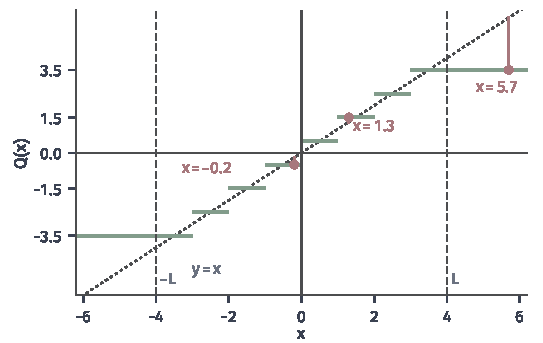
\includegraphics[width=92mm]{figures/07-probability/05-source-coding/matplotlib/quant-uniform-staircase/figure.pdf}
 \caption{$N=8$、$L=4$、$\Delta=1$的均匀量化器。绿线为阶梯$Q(x)$，点线为$y=x$，虚线标出表示范围的两端。红点是读数$1.3$、$-0.2$、$5.7$的输出，红色竖线的长度是误差；范围外的阶梯无限延长，误差随读数线性增大。}
 \label{fig:quant-uniform-staircase}
\end{BookInlineFigure}

\paragraph{有限范围的两种误差}
图中可以分出两种情形。读数在$[-L,L]$内时，它与所在区间的中点相距不超过半个步长，
\[
 \lvert x-Q(x)\rvert\leq\frac{\Delta}{2},\qquad \lvert x\rvert\leq L ;
\]
这部分误差称为\term{舍入误差}（granular error）。读数超出范围时，误差为$\lvert x\rvert-(L-\Delta/2)$，随读数无限增大，称为\term{过载误差}（overload error）。

只要$N$有限而区间都有界，就覆盖不了整条实轴，总要对范围外的读数作某种约定。饱和是最简单的一种。另一种做法是保留一个“越界”索引，再另外描述越界的读数，这等于增加了点数或改变了索引长度，比较时要把这部分资源计入。

两种误差对步长的要求相反。$N$固定时，缩小步长使舍入误差变小，却使范围$L=N\Delta/2$变窄、过载更频繁。对Laplace读数取$N=4$、$\Delta=1$，即$L=2$，重构值为$\pm0.5,\pm1.5$，平均失真为$0.5142$；第~\ref{sec:quant-granular-overload}节将把它分解成两部分，并给出权衡的方法。这个四点量化器也是下一小节迭代的起点。

\subsection{非均匀量化}
\label{sec:quant-nonuniform}

Laplace读数集中在零附近，尾部却延伸得很远。均匀刻度在这里有些浪费：中间密集的地方和尾部稀疏的地方用同样的步长。直观上，概率大的地方应当划得细些，概率小的地方划得粗些。下面固定点数$N$和平方误差，寻找使平均失真最小的区间和重构值。这样构造的量化器一般不等距，称为\term{非均匀量化}（non-uniform quantization）。

同时优化$N-1$个阈值和$N$个重构值并不容易，因为目标对它们的依赖相互纠缠。把变量分成两组，每次固定一组优化另一组，两个子问题都有显式解。

\paragraph{固定区间选重构值}
区间固定后，平均失真按区间拆成互不相关的几块，每块只依赖一个重构值，可以分别优化。于是问题化为：在一个区间上放一个点，使该区间内的平方误差最小。

期望是质量分布的重心，方差是绕重心的转动惯量。把区间$S$上的那部分概率质量看作一块物体，平方误差$\mathbb{E}[(X-c)^2\mathbf{1}_{\{X\in S\}}]$就是它绕点$c$的转动惯量，最好的$c$应当是这块质量的重心。下面的引理把这个直观写成恒等式，它是力学中平行轴定理的概率版本。

\begin{lemma}[质心条件]
\label{lem:quant-centroid}
设$\mathbb{E}[X^{2}]<\infty$，$S$是Borel集且$p=\mathbb{P}(X\in S)>0$，记条件均值
\begin{equation}
 m=\mathbb{E}[X\mid X\in S]=\frac{\mathbb{E}[X\mathbf{1}_{\{X\in S\}}]}{p} .
 \label{eq:quant-conditional-mean}
\end{equation}
则对每个实数$c$，
\begin{equation}
 \mathbb{E}\bigl[(X-c)^{2}\mathbf{1}_{\{X\in S\}}\bigr]=\mathbb{E}\bigl[(X-m)^{2}\mathbf{1}_{\{X\in S\}}\bigr]+p\,(m-c)^{2} .
 \label{eq:quant-parallel-axis}
\end{equation}
因此该区间内的平方误差在$c=m$时唯一地取到最小。
\end{lemma}

\begin{proof}
把$X-c$写成$(X-m)+(m-c)$，平方后展开：
\[
 (X-c)^{2}=(X-m)^{2}+2(m-c)(X-m)+(m-c)^{2} .
\]
两边乘$\mathbf{1}_{\{X\in S\}}$再取期望。二阶矩有限保证每一项都可积。交叉项中，
\[
 \mathbb{E}\bigl[(X-m)\mathbf{1}_{\{X\in S\}}\bigr]=\mathbb{E}[X\mathbf{1}_{\{X\in S\}}]-mp=0 ,
\]
最后一步用了式~\eqref{eq:quant-conditional-mean}。常数项的期望是$p(m-c)^{2}$，于是得到式~\eqref{eq:quant-parallel-axis}。右边第一项与$c$无关，第二项非负且只在$c=m$时为零，所以最小点唯一。
\end{proof}

式~\eqref{eq:quant-parallel-axis}说明，重构值偏离重心的代价是区间概率乘以偏离距离的平方，且与区间内部的分布形状无关。满足这一条件的重构值称为区间的质心。

用第~\ref{chap:conditional-expectation}章的语言，若每个正概率区间的重构值都是质心，则$Q(X)=\mathbb{E}[X\mid J]$，即量化输出是读数在“只知道索引”这一信息下的条件期望，也就是$X$到索引所生成的信息上的正交投影。正交性给出一个计算平均失真的捷径：
\begin{equation}
 D(Q)=\mathbb{E}[X^{2}]-\mathbb{E}\bigl[Q(X)^{2}\bigr]=\mathbb{E}[X^{2}]-\sum_{j=1}^{N}p_jc_j^{2} .
 \label{eq:quant-centroid-distortion}
\end{equation}
它由勾股定理
\[
 \mathbb{E}[X^{2}]=\mathbb{E}\bigl[Q(X)^{2}\bigr]+\mathbb{E}\bigl[(X-Q(X))^{2}\bigr]
\]
得到，只在重构值都是质心时成立。

以Laplace读数为例，看区间$[0,1)$。按$\operatorname{Laplace}(0,1)$的密度直接积分，得到这个区间的概率与一阶矩：
\[
 p=\frac{1-\mathrm{e}^{-1}}{2}=0.3161,\qquad \mathbb{E}[X\mathbf{1}_{\{0\leq X<1\}}]=\frac{1-2\mathrm{e}^{-1}}{2}=0.1321 .
\]
二者相除，质心为
\[
 m=\frac{0.1321}{0.3161}=0.4180 .
\]
它比区间中点$0.5$更靠近零，因为密度在区间内向右递减，质量偏向左端。图~\ref{fig:quant-centroid-nn}左图画出该区间内的平方误差随$c$变化的抛物线：最低点在$m=0.418$，中点$0.5$处的值比最低点多出$p(0.5-0.418)^2=0.0021$。

\begin{BookInlineFigure}
 \centering
 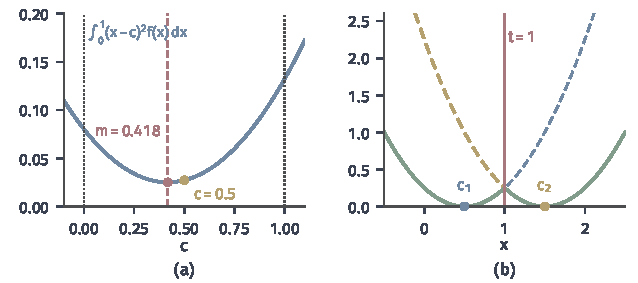
\includegraphics[width=108mm]{figures/07-probability/05-source-coding/matplotlib/quant-centroid-nn/figure.pdf}
 \caption{两个子问题的解。(a) $\operatorname{Laplace}(0,1)$在区间$[0,1)$上的平方误差$\int_0^1(x-c)^2f(x)\,\mathrm{d}x$随$c$的变化（蓝线），最低点在质心$m=0.418$（红点），区间中点$c=0.5$（黄点）处略高。(b) 固定重构值$c_1=0.5$、$c_2=1.5$时，两条虚线是$(x-c_1)^2$与$(x-c_2)^2$，绿线是它们的下包络；两者在中点$t=1$（红线）处交换。}
 \label{fig:quant-centroid-nn}
\end{BookInlineFigure}

\paragraph{固定重构值选区间}
现在反过来，重构值$c_1<\dots<c_N$固定，问每个读数应归入哪个区间。平均失真是逐点误差的期望，而逐点误差只取决于这个读数被报成哪个值。所以对每个读数分别选最近的重构值，就使平均失真最小，不需要考虑其他读数。

\begin{lemma}[最近邻条件]
\label{lem:quant-nearest}
设重构值$c_1,\dots,c_N$固定，$Q$是以它们为重构值的任一量化器。则
\begin{equation}
 D(Q)\geq\mathbb{E}\Bigl[\min_{1\leq k\leq N}(X-c_k)^{2}\Bigr] ,
 \label{eq:quant-nearest-bound}
\end{equation}
等号成立当且仅当以概率$1$有$(X-Q(X))^{2}=\min_k(X-c_k)^{2}$，即几乎每个读数都被报成离它最近的重构值。
\end{lemma}

\begin{proof}
对每个$x$，$Q(x)$是某个$c_k$，所以逐点有$(x-Q(x))^{2}\geq\min_k(x-c_k)^{2}$。两边是非负可测函数，取期望即得式~\eqref{eq:quant-nearest-bound}。两边之差是非负随机变量，它的期望为零当且仅当它几乎必然为零，这就是等号条件。
\end{proof}

最近邻规则下的区间可以直接算出来。对相邻的两个重构值，比较两种误差：
\[
 (x-c_j)^{2}-(x-c_{j+1})^{2}=(c_{j+1}-c_j)\bigl(2x-c_j-c_{j+1}\bigr) .
\]
由于$c_{j+1}>c_j$，左边小于零当且仅当$x$小于两点的中点。所以最近邻区间仍是区间，阈值是相邻重构值的中点：
\begin{equation}
 t_j=\frac{c_j+c_{j+1}}{2},\qquad j=1,\dots,N-1 .
 \label{eq:quant-midpoint-threshold}
\end{equation}
读数恰好落在中点时两个重构值一样近，需要约定归属，例如归入编号较小的一个。对有密度的读数，中点的概率为零，约定不影响平均失真。图~\ref{fig:quant-centroid-nn}右图画出两条误差抛物线和它们的下包络，交点就在中点$t=1$。

\paragraph{两条必要条件}
两个引理合起来，就是最优量化器必须满足的条件。

\begin{theorem}[Lloyd--Max条件]
\label{thm:quant-lloyd-max-conditions}
设$\mathbb{E}[X^{2}]<\infty$，平方误差下$Q^{*}$在所有$N$点量化器中平均失真最小，其区间为$S_j$、重构值为$c_j$。则：
\begin{enumerate}
 \item 对每个$p_j=\mathbb{P}(X\in S_j)>0$，$c_j=\mathbb{E}[X\mid X\in S_j]$；
 \item 以概率$1$有$(X-c_{\alpha(X)})^{2}=\min_k(X-c_k)^{2}$。
\end{enumerate}
\end{theorem}

\begin{proof}
若第一条对某个$j$不成立，由引理~\ref{lem:quant-centroid}，把$c_j$换成条件均值严格减小区间$S_j$上的误差，其余区间不变，平均失真严格下降，与$Q^{*}$最优矛盾。若第二条不成立，由引理~\ref{lem:quant-nearest}，保持重构值、按最近邻重新划分，平均失真严格下降，同样矛盾。
\end{proof}

这两条只是必要条件，不是充分条件：满足它们的量化器可能不是最优的，后面会给出例子。定理也没有断言最优量化器存在。对平方误差和二阶矩有限的读数，$N$点最优量化器确实存在：离分布太远的重构值可以拉回而不增大失真，于是只需在有界的重构值集合中寻找，再用紧性论证取到最小值。下面的迭代只用到两条必要条件，不依赖存在性。

\paragraph{交替改进的思想}
两条条件提示了一个迭代：从某组重构值出发，先按式~\eqref{eq:quant-midpoint-threshold}取中点作阈值，再按式~\eqref{eq:quant-conditional-mean}把每个重构值移到新区间的质心，然后重复。每一步都是在固定另一组变量时求得的最优解，所以平均失真不会上升。这种做法称为\term{Lloyd--Max算法}（Lloyd--Max algorithm）。写成公式，第$t$轮的两步为
\begin{equation}
 t_j^{(t)}=\frac{c_j^{(t-1)}+c_{j+1}^{(t-1)}}{2},\qquad
 c_j^{(t)}=\mathbb{E}\bigl[X\bigm| t_{j-1}^{(t)}\leq X<t_j^{(t)}\bigr] ,
 \label{eq:quant-lloyd-update}
\end{equation}
其中$t_0^{(t)}=-\infty$、$t_N^{(t)}=+\infty$。

对Laplace读数，质心有显式形式，迭代可以手算。$\operatorname{Laplace}(0,1)$在$x\geq0$上就是$\frac12\mathrm{e}^{-x}$，对$0\leq a<b$，积分得到区间的概率与条件均值：
\begin{equation}
 \begin{gathered}
 \mathbb{P}(a\leq X<b)=\frac{\mathrm{e}^{-a}-\mathrm{e}^{-b}}{2},\\
 \mathbb{E}[X\mid a\leq X<b]=\frac{(a+1)\mathrm{e}^{-a}-(b+1)\mathrm{e}^{-b}}{\mathrm{e}^{-a}-\mathrm{e}^{-b}} .
 \end{gathered}
 \label{eq:quant-laplace-centroid}
\end{equation}
令$b\to\infty$，得到$\mathbb{E}[X\mid X\geq a]=a+1$：超过$a$的部分服从$\operatorname{Exp}(1)$，均值为$1$，这是指数分布无记忆性的直接结果。负半轴由对称性得到。

\paragraph{计算过程}
下面用$N=4$、从上一小节的均匀量化器出发，逐轮演示。读数分布关于零对称，初始重构值也对称，每轮更新后仍对称，所以中间阈值始终为$0$，只需跟踪正半轴的一个阈值和两个重构值。

\needspace{6\baselineskip}
\paragraph{变量}
\begin{itemize}
 \item $c_1^{(t)}<\dots<c_N^{(t)}$：第$t$轮的重构值，共$N$个实数。
 \item $t_1^{(t)}<\dots<t_{N-1}^{(t)}$：第$t$轮的阈值，共$N-1$个实数，两端补$\pm\infty$。
 \item $D^{(t)}$：第$t$轮量化器的平均失真，用于判断何时停止。
\end{itemize}
例中由对称性，只需记录$t_3^{(t)}$、$c_3^{(t)}$与$c_4^{(t)}$。

\paragraph{初始化}
重构值初始化为一组互不相同的点，常用的选择是同样点数的均匀量化器，或者从源分布中抽取的几个值。$D^{(0)}$是这组点配上最近邻区间时的平均失真。例中取$\Delta=1$的均匀量化器，
\[
 c^{(0)}=(-1.5,\,-0.5,\,0.5,\,1.5),\qquad D^{(0)}=0.5142 .
\]

\needspace{6\baselineskip}
\paragraph{每轮更新}
在第$t$轮：
\begin{enumerate}
 \item \textbf{更新阈值。}按式~\eqref{eq:quant-lloyd-update}的第一式取相邻重构值的中点。例中第一轮
 \[
  t_3^{(1)}=\frac{0.5+1.5}{2}=1 ,
 \]
 阈值为$(-1,0,1)$，与初始量化器相同。

 \item \textbf{更新重构值。}按式~\eqref{eq:quant-lloyd-update}的第二式把每个重构值移到新区间的质心，Laplace读数用式~\eqref{eq:quant-laplace-centroid}计算。例中第一轮内侧区间是$[0,1)$，外侧是$[1,\infty)$：
 \[
  c_3^{(1)}=\frac{1-2\mathrm{e}^{-1}}{1-\mathrm{e}^{-1}}=0.4180,\qquad c_4^{(1)}=1+1=2 .
 \]
 外侧的重构值从$1.5$跳到$2$：尾部质量的重心比区间起点远一个单位。

 \item \textbf{计算平均失真。}重构值已是质心，可用式~\eqref{eq:quant-centroid-distortion}，其中$\mathbb{E}[X^2]=2$。例中两侧区间概率为$0.3161$和$0.1839$，
 \[
  D^{(1)}=2-2\bigl(0.3161\times0.4180^{2}+0.1839\times2^{2}\bigr)=0.4180 .
 \]

 \item \textbf{判断停止。}若相对下降$(D^{(t-1)}-D^{(t)})/D^{(t)}$小于预先给定的$\varepsilon$，停止；否则进入下一轮。例中取$\varepsilon=10^{-3}$，第一轮下降约$23\%$，继续。
\end{enumerate}

例中第二轮先取中点，
\[
 t_3^{(2)}=\frac{0.4180+2}{2}=1.2090 .
\]
再计算新区间的质心。由$\mathrm{e}^{-1.209}=0.2985$与式~\eqref{eq:quant-laplace-centroid}，
\[
 c_3^{(2)}=\frac{1-2.209\times0.2985}{1-0.2985}=0.4856,\qquad c_4^{(2)}=2.2090 .
\]
内侧区间概率为$(1-0.2985)/2=0.3508$，外侧为$0.1492$，于是
\[
 D^{(2)}=2-2\bigl(0.3508\times0.4856^{2}+0.1492\times2.209^{2}\bigr)=0.3781 .
\]

以后各轮照此进行。表~\ref{tab:quant-lloyd-rounds}列出前八轮的结果。阈值和外侧重构值每轮外移，内侧重构值在第一轮内移后也逐步外移，平均失真单调下降。

\begin{BookInlineTable}
 \centering
 \begin{tabular}{ccccc}
  \toprule
  $t$ & $t_3^{(t)}$ & $c_3^{(t)}$ & $c_4^{(t)}$ & $D^{(t)}$\\
  \midrule
  $0$ & $1.0000$ & $0.5000$ & $1.5000$ & $0.5142$\\
  $1$ & $1.0000$ & $0.4180$ & $2.0000$ & $0.4180$\\
  $2$ & $1.2090$ & $0.4856$ & $2.2090$ & $0.3781$\\
  $3$ & $1.3473$ & $0.5268$ & $2.3473$ & $0.3624$\\
  $4$ & $1.4370$ & $0.5521$ & $2.4370$ & $0.3563$\\
  $5$ & $1.4945$ & $0.5677$ & $2.4945$ & $0.3539$\\
  $6$ & $1.5311$ & $0.5774$ & $2.5311$ & $0.35299$\\
  $7$ & $1.5543$ & $0.5835$ & $2.5543$ & $0.35263$\\
  $8$ & $1.5689$ & $0.5873$ & $2.5689$ & $0.35248$\\
  \midrule
  $\infty$ & $1.5936$ & $0.5936$ & $2.5936$ & $0.35239$\\
  \bottomrule
 \end{tabular}
 \caption{$\operatorname{Laplace}(0,1)$、$N=4$的Lloyd--Max迭代，只列正半轴；第$0$行是初始的均匀量化器，末行是不动点。}
 \label{tab:quant-lloyd-rounds}
\end{BookInlineTable}

第七轮的相对下降为$(0.35299-0.35263)/0.35263\approx1.02\times10^{-3}$，尚未达标；第八轮为$(0.35263-0.35248)/0.35248\approx4.3\times10^{-4}$，迭代停止。最终得到的量化器为
\[
 \begin{gathered}
 t=(-1.569,\ 0,\ 1.569),\qquad D=0.3525,\\
 c=(-2.569,\ -0.587,\ 0.587,\ 2.569) .
 \end{gathered}
\]
比初始的均匀量化器的$0.5142$减少约$31\%$，点数没有变。

迭代的极限可以单独求出，用来检验上面的结果。由式~\eqref{eq:quant-laplace-centroid}，外侧质心总是$c_4=t+1$；不动点处阈值是中点，$t=(c_3+c_4)/2$，于是$c_3=t-1$。再要求$c_3$是$[0,t)$的质心，得到关于$t$的方程
\[
 t-1=\frac{1-(t+1)\mathrm{e}^{-t}}{1-\mathrm{e}^{-t}} .
\]
它的正根为$t=1.5936$，相应$c_3=0.5936$、$c_4=2.5936$，由式~\eqref{eq:quant-centroid-distortion}得$D=0.3524$。图~\ref{fig:quant-lloyd-rounds}画出迭代二十轮的轨迹，各量都向这个不动点靠拢。

\begin{BookInlineFigure}
 \centering
 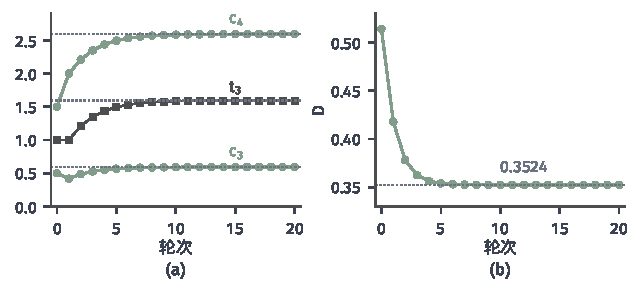
\includegraphics[width=108mm]{figures/07-probability/05-source-coding/matplotlib/quant-lloyd-rounds/figure.pdf}
 \caption{$\operatorname{Laplace}(0,1)$、$N=4$的Lloyd--Max迭代。(a) 正半轴的阈值$t_3$（灰色方块）与重构值$c_3$、$c_4$（绿色圆点）随轮次的变化，点线为不动点。(b) 平均失真随轮次单调下降，点线为不动点处的$0.3524$。}
 \label{fig:quant-lloyd-rounds}
\end{BookInlineFigure}

\paragraph{目标单调下降}
记$D(\mathcal{S},\bm{c})$为区间组$\mathcal{S}$配重构值$\bm{c}$时的平均失真。第$t$轮先由引理~\ref{lem:quant-nearest}，再由引理~\ref{lem:quant-centroid}，得到
\[
 D\bigl(\mathcal{S}^{(t)},\bm{c}^{(t)}\bigr)\leq D\bigl(\mathcal{S}^{(t)},\bm{c}^{(t-1)}\bigr)\leq D\bigl(\mathcal{S}^{(t-1)},\bm{c}^{(t-1)}\bigr) .
\]
所以$D^{(t)}$单调不增。它有下界$0$，因此收敛。

这个论证只说明平均失真的数值收敛，没有说明阈值和重构值本身收敛，更没有说明收敛到最优量化器。例中参数也收敛了，那是这个具体分布的性质。

每轮的代价是计算$N$个区间的概率与一阶矩。分布有显式的积分公式时，代价与$N$成正比；需要数值积分或模拟时，还要加上积分误差，这一点在第~\ref{sec:quant-granular-overload}节再谈。

\paragraph{初始化、空区间与并列}
初始重构值必须互不相同，否则两个点的最近邻区间无法区分。迭代中若某个区间的概率为零，它的条件均值没有定义，式~\eqref{eq:quant-lloyd-update}无法执行。对Laplace这样处处有正密度的读数，只要重构值互不相同，每个区间都有正概率，这种情况不会发生；对离散读数或支撑有空隙的读数则可能发生。常见的处理是保留原来的重构值，或者把它挪到当前误差最大的区间内，把那个区间一分为二。前一种做法仍保证目标不增，后一种改变了迭代的路线，需要重新检查单调性。

读数恰好落在两个重构值的中点时，两者一样近。对有密度的读数，这个事件概率为零；对离散读数，归属约定会改变区间的质心，从而改变后续的迭代，所以必须事先固定，例如一律归入编号较小的区间。

\paragraph{局部最优}
目标下降并不保证到达全局最小。考虑一个离散读数，等概率地取$0$、$2$、$3.5$三个值，用$N=2$个点量化。有两种不同的划分都满足Lloyd--Max条件。

第一种把$\{0\}$与$\{2,3.5\}$分开，重构值是两组的平均：
\[
 c=(0,\ 2.75),\qquad t=1.375 .
\]
$2$离$2.75$比离$0$近，划分与最近邻一致，是不动点。平均失真为
\[
 D=\frac{0+0.75^{2}+0.75^{2}}{3}=0.375 .
\]

第二种把$\{0,2\}$与$\{3.5\}$分开，
\[
 c=(1,\ 3.5),\qquad t=2.25 .
\]
$2$离$1$的距离是$1$，离$3.5$是$1.5$，仍归第一组，也是不动点。平均失真为
\[
 D=\frac{1+1+0}{3}=0.667 .
\]

从$c^{(0)}=(0,1)$出发，阈值$0.5$给出第一种划分；从$c^{(0)}=(1,4)$出发，阈值$2.5$给出第二种划分。两次迭代都在第一轮后停住，结果相差近一倍。图~\ref{fig:quant-lloyd-local}画出这两个不动点。

\begin{BookInlineFigure}
 \centering
 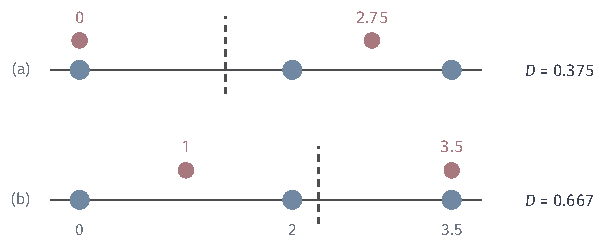
\includegraphics[width=102.5mm]{figures/07-probability/05-source-coding/tikz/quant-lloyd-local/figure.pdf}
 \caption{等概率取$0$、$2$、$3.5$（蓝点）的读数用两个点量化时的两个Lloyd--Max不动点。红点为重构值，虚线为阈值。(a) 划分$\{0\}$、$\{2,3.5\}$，$D=0.375$，是全局最优；(b) 划分$\{0,2\}$、$\{3.5\}$，$D=0.667$，也满足两条必要条件，但不是最优。}
 \label{fig:quant-lloyd-local}
\end{BookInlineFigure}

所以实际计算中常从多组初始值出发，保留平均失真最小的结果。对一维有密度的读数，若密度的对数是凹函数（Laplace与高斯都满足），满足两条条件的量化器只有一个，Lloyd--Max迭代因而收敛到全局最优。证明要说明不动点方程组只有一个解，需要逐个比较阈值的单调性，篇幅较长；上面Laplace例子的不动点方程只有一个正根，与这一结论相符。

\paragraph{与均匀量化的比较}
同样的迭代可以用于任意点数。图~\ref{fig:quant-lloydmax-vs-uniform}比较$N=8$时Lloyd--Max的不动点与最好的均匀量化器（步长在所有$\Delta$中搜索得到）。Lloyd--Max的区间在中央最窄、向外逐渐变宽，最外侧的重构值远达$\pm4.37$；均匀量化器的步长约为$1.03$，范围只到$\pm4.13$。两者的平均失真分别为$0.1090$与$0.1435$，在同样$3$个比特下，按分布调整的划分把误差降低了约$24\%$。

\begin{BookInlineFigure}
 \centering
 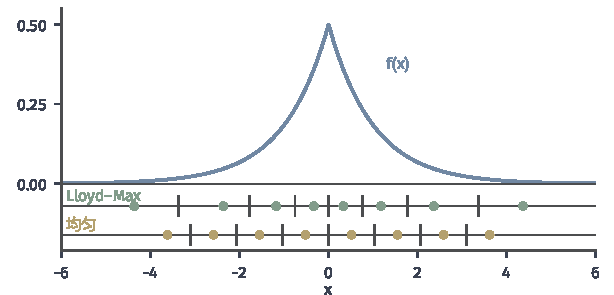
\includegraphics[width=104mm]{figures/07-probability/05-source-coding/matplotlib/quant-lloydmax-vs-uniform/figure.pdf}
 \caption{$\operatorname{Laplace}(0,1)$的两个8点量化器。蓝线为密度。上一行绿点为Lloyd--Max不动点的重构值，竖线为阈值；下一行黄点为最好的均匀量化器的重构值（步长约$1.03$）。Lloyd--Max在中央划得更细、在尾部划得更粗。}
 \label{fig:quant-lloydmax-vs-uniform}
\end{BookInlineFigure}

代价在实现上。均匀量化的编码器按式~\eqref{eq:quant-uniform-encoder}一次除法和取整就能完成，非均匀量化则要把读数与$N-1$个阈值比较（二分查找需要约$\log_2N$次比较），并且需要知道源分布才能设计。
